% Name: Lorenz curve and Gini coefficient
% Description: The share of income held by the poorest fraction of people, against the line of perfect equality: the Gini coefficient is the gap A as a share of A plus B.
% Tags: Lorenz curve, Gini coefficient, inequality, income distribution

\begin{tikzpicture}[scale=5, every node/.style={font=\small}]
  % L(p) = p², so B = ∫ p² dp = 1/3, A = 1/2 - 1/3 = 1/6, and G = A / (A + B) = 1/3
  \fill[orange!25] (0,0) -- (1,1) -- plot[domain=1:0, samples=40] (\x, {\x*\x}) -- cycle;
  \fill[blue!15] (0,0) -- plot[domain=0:1, samples=40] (\x, {\x*\x}) -- (1,0) -- cycle;
  \draw[thick] (0,0) rectangle (1,1);
  \draw[thick, gray] (0,0) -- (1,1);
  \draw[very thick, blue!70!black] plot[domain=0:1, samples=40] (\x, {\x*\x});
  \node at (0.45,0.33) {$A$};
  \node at (0.72,0.2) {$B$};
  \node[rotate=45, above, font=\footnotesize, gray!40!black] at (0.3,0.3) {perfect equality};
  \node[rotate=40, below right, font=\footnotesize, blue!60!black] at (0.62,0.38) {Lorenz curve};
  \foreach \t in {0, 0.5, 1} \node[below] at (\t,0) {$\t$};
  \foreach \t in {0.5, 1} \node[left] at (0,\t) {$\t$};
  \node[below=4mm] at (0.5,0) {share of people, poorest first};
  \node[rotate=90, above=5mm] at (0,0.5) {share of income};
  \node[anchor=west] at (1.05,0.5) {$G = \dfrac{A}{A + B} = \dfrac{1}{3}$};
\end{tikzpicture}
